\documentclass[oneside]{article}
\usepackage{graphicx}
\usepackage[pagebackref]{hyperref}
\usepackage[section]{placeins}

\author{Submitter: Srirang Sarpotdar-Sairamulu}
\title{Proposal for New Emoji: PEAS}
\date{Date: 15th August 2021}

\begin{document}
\renewcommand{\thesubsection}{\thesection.\Alph{subsection}}
\renewcommand{\thesubsubsection}{\thesubsection.\alph{subsubsection}}
\maketitle

\tableofcontents
\label{contents}
\newpage

\abstract
This proposal seeks the addition of an emoji for peas, an almost universally
known vegetable (technically fruit) that forms an important part of many
culinary traditions across the world. As far as I know, an emoji for peas does
not exist and I think it would be of significant value as an addition to the
Emoji standard.

\section{Identification}
A.  CLDR short name: PEAS

\noindent
B.  CLDR keywords: PEAS, POD

\section{Images}
//gather and attach images

\section{Category}
//set category

\section{Introduction}
The small spherical seed in the seed-pod of \textit{P. Sativum} is commonly known
as the pea, although the plant and the seed-pod are themselves often called
peas as well. Originating in the Mediterranean basin, the modern pea is the
result of continuous selection stretching back to the Neolithic period. Peas
feature in the historical record as well, with Theoprastus in the 3rd Century
BCE mentioning that peas are sown in the late winter owing to their tenderness.
In the Middle Ages, peas developed into a staple that kept famine at bay, as
Charles the Good, Count of Flanders noted in 1124.

Today peas are both a celebrated ingredient in many foods as well as an instantly recognizable motif that merits the inclusion of PEAS (the proposed emoji) into the Emoji standard.

\section{Selection Factors - Inclusion}

\subsection{Compatibility}
To the best of my knowledge no platform supports any form of PEAS at
the time of writing but its addition would go towards both completiing the
existing set of emoji as well as adding to the emoji lexicon in general.

\subsection{Expected Usage Level}

\subsubsection{Frequency}

\begin{figure}[!htb]
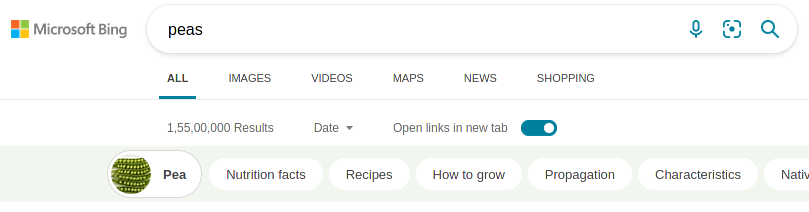
\includegraphics[width=12cm]{bing.png}
\caption{Bing Search Results (1,55,00,000 hits)}
\label{fig:bing}
\end{figure}

\begin{figure}[!htb]
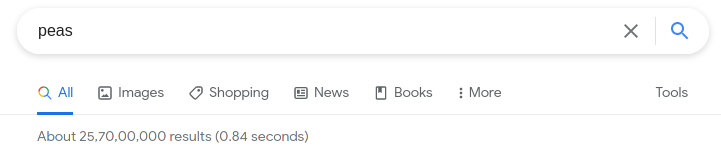
\includegraphics[width=12cm]{google.png}
\caption{Google Search Results (25,70,00,000 hits)}
\label{fig:google}
\end{figure}

\begin{figure}[!htb]
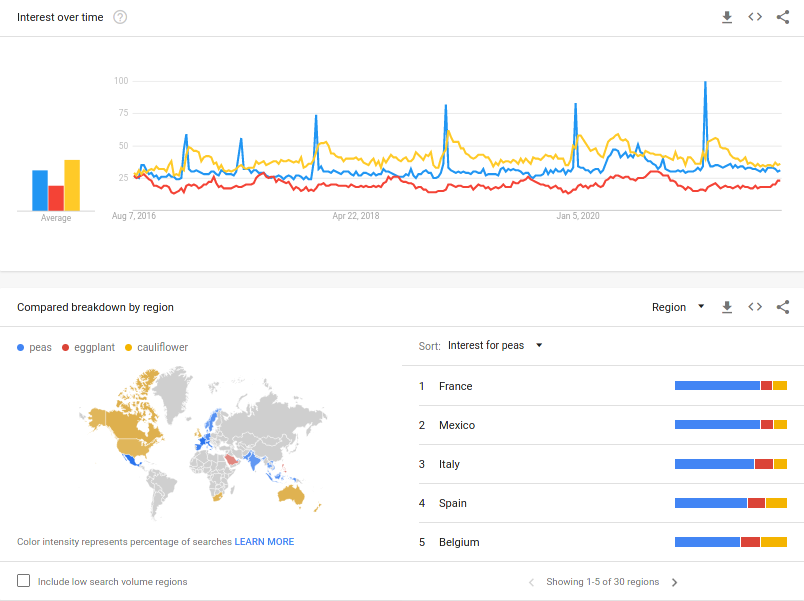
\includegraphics[width=12cm]{analytics.png}
\caption{Google Search Trends comparsion with relevant existing emoji}
\label{fig:google}
\end{figure}


\subsubsection{Multiple Usages}
Apart from its culinary usage, the phrase "peas in a pod" describes a strong
similarity between people. Due to its visual proximity with the generic imagery
of beans, it can also be used in "cool beans" as well. There is a possibility of
it being used as a pun on the word "peace".

\subsubsection{Use in sequences}
n/a

\subsubsection{Breaking new ground}
This submission does not break new ground in that it seeks to expand the
fruits/vegetables categories by adding a much needed new member. However, if
added it would be the first emoji to represent a sort of bean.

\subsection{Distinctiveness}
PEAS is both visually and semantically distinct from the existing
fruit/vegetable emoji. The imagery of 3 peas in an open pod is familiar to most
viewers and is instantly recognizable even at the typically small sizes emoji
are displayed in.

\subsection{Completeness}
Despite peas being ubiquitous as both imagery and food, the Emoji standard does
not include them under Fruits or Vegetables. Adding a pea emoji would go
towards completing either and filling an existing gap.

\section{Selection Factors - Exclusion}

\subsection{Petitions or “frequent requests”}
//address dumbass petitions

\subsection{Overly specific}
While adding to the fruit/vegetable category, PEAS would represent a new
category (i.e. beans) within the emoji lexicon and so are not overly specific.

\subsection{Open-ended}
As there are currently no related emoji in place currently, PEAS would be
unique therefore not result in the need to add more such emojis.

\subsection{Already representable}
To the best of my knowledge, peas are not representable with any sequence of
emoji, normal or ZWJ.

\subsection{Logos, brands, other third-party IP rights, UI icons, signage, specific people, specific buildings and landmarks, deities}
The proposed emoji is none of the above.

\subsection{Transient}
The history of peas is well-attested to and the need for inclusion of PEAS does
not arise out of any fad or meme but out of a genuine necessity to fill a gap
in the emoji lexicon.

\subsection{Faulty comparison}
n/a

\subsection{Exact images}
The imagery used is generic yet immediately recognizable and does not require
precise/exact images to convey the full scope of meaning.

\subsection{Region flags without code}
n/a

\subsection{Lack of required rights or license for images}
n/a

\subsection{Variations on direction}
n/a

\subsection{Includes text}
n/a

\end{document}



